\documentclass[aps,pre,12pt,preprint,%
	onecolumn,showpacs,showkeys,nofootinbib]{revtex4-1}
%Chinese
	\usepackage[UTF8,fontset=fandol]{ctex}
	\xeCJKsetup{underdot = {
		boxdepth=0pt, format=\huge, depth=.4em
	}}
%	\usepackage[datesep=/]{datetime2} % Use default
	\DeclareTextFontCommand{\textbf}{\sffamily}
%Presenting
	\usepackage[table]{xcolor}
	\usepackage{graphicx}
	\usepackage[space]{grffile}
	\usepackage[font=small,format=plain,%
		labelfont=bf,textfont=it,%
		singlelinecheck=false]{caption}
	\usepackage[above]{placeins}
%	\usepackage{float} % Cause trouble for table footnotes
	\usepackage{wrapfig}
	\usepackage{tabularx,array,booktabs,multirow,bigstrut}
	\newcolumntype{C}[1]{>{\hsize=#1\hsize%
		\centering\arraybackslash}X}
	\newcommand{\minitab}[2][l]{%
		\begin{tabular}{#1}#2\end{tabular}}
	\usepackage{setspace,dcolumn}
	\usepackage{subfig}
	\usepackage{psfrag,epsfig}
%MathSetting
	\let\latexointop\ointop
	\usepackage{amsmath,bm,amssymb,esint,extarrows}
	\usepackage{upgreek,textcomp,mathrsfs}
	\usepackage[only,sslash]{stmaryrd}
	\usepackage{nicefrac,eqnarray}
%	\usepackage{amsthm} % Enable when necessary
%	\usepackage[mathscr]{eucal} % Enable when necessary
	\usepackage{mathtools,physics,siunitx}
	\usepackage{stackengine,varwidth}
	\usepackage{tikz}
	\usepackage{resizegather,empheq}
	\usetagform{default}
	\usepackage{calligra,fourier-orns}
	% Keep \oint unchanged by esint
	\let\ointop\undefined
	\let\ointop\latexointop
	% Define a scriptr 
	\DeclareMathAlphabet{\mathcalligra}{T1}{calligra}{m}{n}
	\DeclareFontShape{T1}{calligra}{m}{n}{<->s*[2.2]callig15}{}
	\newcommand{\scriptr}{\mathcalligra{r}\,}
	\newcommand{\rvector}{\pmb{\mathcalligra{r}}\,}
	% Useful shorthand
	\DeclarePairedDelimiter\ave{\langle}{\rangle}
	\newcommand\inlineeqno{\stepcounter{equation}\ (\theequation)}
	\newcommand{\sinc}{\operatorname{sinc}}
	\newcommand{\mbb}[1]{\mathbb{#1}}
	\newcommand{\mrm}[1]{\mathrm{#1}}
	\newcommand{\mcal}[1]{\mathcal{#1}}
	\newcommand{\tup}[1]{\textup{#1}}
	% Scaling and positioning
	\newcommand\scalemath[2]{\scalebox{#1}{\mbox{\ensuremath{\displaystyle #2}}}}
	\newcommand\raisemath[2]{\raisebox{#1\depth}{${#2}$}}
	\empheqset{box=\nicebox}
	% Presenting
	\newcommand*\nicebox[1]{\fbox{\hspace{1em}\addstackgap[5pt]{#1}\hspace{1em}}}
	\sisetup{%
		redefine-symbols=false,%
		separate-uncertainty=true,%
		range-phrase=\,\textasciitilde\,,%
		arc-separator = \,}
	\allowdisplaybreaks[2]
%ParagraphSetting
	\setlength{\parskip}{.3\baselineskip}
	\usepackage[defaultlines=2,all]{nowidow}
	\postdisplaypenalty=50
%PageSetting
	\usepackage{titlesec}
	\titleformat*{\section}{\large\bfseries}
	\usepackage[colorlinks=true,linkcolor=blue]{hyperref}
	\newcommand{\texstringonly}[1]{%
		\texorpdfstring{#1}{}}
	\usepackage[vmargin={3.5cm,4cm},hmargin=3cm,%
		footnotesep=\baselineskip]{geometry}
%	\usepackage[bottom]{footmisc} % Cause trouble for table footnotes
	\usepackage{changepage}
	% Autoref names
	\renewcommand{\tableautorefname}{\tablename}
	\renewcommand{\figureautorefname}{\figurename}
	% List settings
	\usepackage{enumitem}
	\setlist{itemsep=0pt,topsep=0pt,labelindent=\parindent,leftmargin=0pt,itemindent=*}
	% Some redefined lengths
	\setlength{\headsep}{1.6\baselineskip}
%	\setlength{\footnotesep}{3\parskip} % Use when necessary
	% Header
	\usepackage{fancyhdr,lastpage}
	\pagestyle{fancy}
%	\fancyhf{} % Clear default settings; disabled for now
	\cfoot{--\ \thepage\,/\,\pageref{LastPage} \ --}
	\setlength{\footskip}{2\baselineskip}
	\renewcommand{\headrulewidth}{0.1pt}
	\renewcommand{\headrule}{
		\ifnum\value{page}=1\relax\else
			\vbox to 2pt{
			\hbox to \headwidth{\dotfill}\vss}
		\fi}
	\fancypagestyle{titlepagestyle}{%
		\fancyhead{}
		\chead{
			\vspace{2.5\baselineskip}
			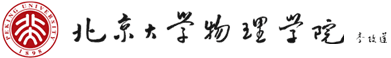
\includegraphics[width=.75\linewidth]{../PKUPhy}}
	}
	% Separator
	\newcommand{\newparagraph}{\pagebreak[3]\noindent%
		\hfil
		~\raisebox{-4pt}[10pt][10pt]{\decofourright~~~~~~~~\decofourleft}~ %
		\par
	}
%	% Background % Use when necessary
%	\usepackage{background} %Waterstamp package
%	\SetBgContents{...的实验报告} %Waterstamp to prevent copying
%	\SetBgScale{5} %Waterstamp setting
	% Essay format
	\renewcommand\appendixname{附录}
	\renewcommand\abstractname{}%摘要
	\renewcommand\tablename{表}
	\renewcommand\figurename{图}
	\renewcommand\refname{参考文献}
	\makeatletter
	\def\@pacs@name{\songti\zihao{-4}{\bf PACS码:}}
	\def\@keys@name{\songti\zihao{-4}{\bf 关键词:}}
	\def\Dated@name{日期:}
	\def\Received@name{\zihao{-5}{接收} }
	\def\Revised@name{\zihao{-5}{修订} }
	\def\Accepted@name{\zihao{-5}{采纳} }
	\def\Published@name{\zihao{-5}{发表} }
	\makeatother
	\linespread{1.5}
	\renewcommand{\labelenumi}{\alph{enumi}.}
	\leftmargini=20mm
	\newcommand{\supercite}[1]{\textsuperscript{\,%
		[\citenum{#1}]}}
	\let\fancycite\cite
	\renewcommand{\cite}[1]{\textup{\fancycite{#1}}}
	% Math line spacing
	\newlength{\djot}
	\setlength{\djot}{\jot}
	\newcommand{\restorejot}{\setlength{\jot}{\djot}}

%Miscellaneous
%	\newcommand{\tabindent}{\hspace{2em}}
%FourierTransform
	\newcommand{\fourierf}{\mathscr F}
%Atoms
	\newcommand{\SrAtom}{\,\textsuperscript{90}\tup{Sr}\,}
	\newcommand{\Yatom}{\,\textsuperscript{90}\tup{Y}\,}
	\newcommand{\CsAtom}{\,\textsuperscript{137}\tup{Cs}\,}
	\newcommand{\CoAtom}{\,\textsuperscript{60}\tup{Cs}\,}
\begin{document}
%Basic Data
	\title{%
	\texstringonly{\hfil\\[2\baselineskip]}
	\sf\LARGE%
		p型硅的电阻率与霍尔系数之测定%
	\texstringonly{\vspace{3ex}}}
	\author{\fangsong\large%
		Bryan%
	\vspace{2mm}}
	\affiliation{\it%
		北京大学物理学院~~学号:\normalfont 1500000000\,}
	\date{\today}
	\keywords{半导体,p型硅,能带理论,霍尔效应,范德堡法}
	\email{guesswhat@email.addr;}

\begin{abstract}
\vspace{10mm}
\begin{spacing}{1.5}\normalsize
\setlength{\parskip}{.3\baselineskip}
%	200—300字,
%	说明用什么方法做了什么事,
%	由此得到什么结果和结论,
%	有何意义.
%	不用缩略词,不用第一人称.
%%%%%%%%%%%%%%%%%%%%%%%%%%%%%%%%
	测定导体的电阻率和霍尔系数,可以获知其基本电学特性,有助于我们了解或验证其导电机理。本实验将这一办法应用到了半导体的研究中,试图通过测定p型硅的电阻率和霍尔系数,验证半导体的导电特性和机理。
	
	具体而言,本实验利用四线范德堡法测量了从室温至$\sim\SI{150}{\celsius}$范围内p型硅的电阻率和霍尔系数,获得并分析了该温度范围内霍尔系数和电阻率对温度的依赖关系;这验证了固体理论对掺杂半导体之导电机制的预测,并进一步给出了所用样品p~型硅的禁带宽度$E_g \sim \SI{1.2}{\eV}$.
\end{spacing}
\end{abstract}

\maketitle
\thispagestyle{titlepagestyle}

%	\item 课程实验报告应假定读者既不是已知全部实验细节的指导教师,也不是缺少专业知识的公众,而是同领域的实验研究者,或审稿人. 不能要求读者要在读过课程讲义后才能读懂课程实验报告.
%	\item 公式、图和表要分别用阿拉伯数字编列序号. 公式和图表要达到可发表的质量.
%	\item 凡不是自己独立思考得到的内容都应该引参考文献. 不能大段引用同一参考文献. 对复杂问题,应该优先考虑引用参考文献得到结果. 对简单一些的问题才鼓励独立思考.
%	\item 较长的推导和说明可以作为附件提交,不占用报告篇幅.
%	\item 思考题不是报告的组成部分. 应另起一页附在报告的最后.
\section{引言}
%%	研究论文引言一般包含以下内容:
%%	(1)所研究领域背景和现状;
%%	(2)有待研究的问题;
%%	(3)本研究的目的、主要内容和结果;
%%	(4)结果的意义.\par
%%	在写实验报告的引言时,同学可以假想自己是第一个做类似研究的人.\par
%%	引言一定要切合报告正文,不能漫无目的地介绍背景. 要快速地将读者引导到报告主题上,并作较深入的讨论.\par
%%	引言篇幅可以在较大范围内变化,但最长不应超过报告文字篇幅的1/3.\par
%%	引言撰写可以参考实验讲义,可以复述,但不能复制讲义上的任何一句话.\par
%%%%%%%%%%%%%%%%%%%%%%%%%%%%%%%
	对半导体的认识和理解源自其电学特性的实验测定。早在19世纪初,人们便观察到了半导体的若干非同寻常的性质;特别是其电阻可能随温度增高而下降,这与寻常的导体截然不同\supercite{lukasiak2010history}。
	
	1878年,霍尔(Edwin Herbert Hall)指出,磁场会导致导体中的载流子发生偏转,电荷在导体侧面累积产生可测的电压,电压正负取决于载流子类型;此即\textit{霍尔效应}\supercite{hall1879new}。随后的1897年,J. J. 汤姆逊(Sir Joseph John Thomson)发现电子\supercite{thomson1897discovery},结合霍尔效应的结论,人们自然猜想,导体中的电流由电子定向漂移形成。
	
	然而,德国物理学家Karl Baedeker首先发现,半导体\tup{CuI}的霍尔现象与导体并不一致;两者的霍尔电压符号相反,且虽说半导体的电导率(\textit{电阻率的倒数})显著低于导体,但其霍尔效应的强度(\textit{以霍尔系数衡量})却显著高于导体\supercite{lukasiak2010history}。Baedeker指出,与导体不同,\tup{CuI}应当具有正电荷载流子;但人们并不清楚这一正电荷载流子究竟由何种粒子构成。
	
	20世纪上半叶发展起来的量子力学及固体理论给上述半导体中的“未解之谜”提供了一个统一的答案。1928年,布洛赫(Felix Bloch)成功地从\textit{波动观点}出发,重新理解了电子在晶格中的运动\supercite{bloch1928quantum};1930年,B. Gudden指出了杂质散射对半导体电导的重要影响\supercite{gudden1930elektrischen};1931年,由威尔逊(Alan Herries Wilson)等人提出的\textit{能带理论}得以确立,统一地解释了导体和半导体的导电特性\supercite{wilson1931theory}。
	
	固体理论解释了半导体在室温附近的不寻常现象,同时还预测了更广温度范围内其电阻及霍尔系数更为丰富的变化规律。本实验考察室温以上直到$\sim\SI{150}{\celsius}$范围内p型硅半导体的电阻率及霍尔系数,确定材料的载流子类型和浓度,从而检验固体理论给出的预测;在此基础上,进一步确定禁带宽度(又称\textit{带隙}或\textit{能隙}),净杂质浓度以及迁移率等多种关于材料导电性的基本参数。
\section{理论}
	固体理论认为半导体的导电机制分为两种,
	\begin{enumerate}[noitemsep]
	\item \textit{本征导电}:由半导体自身晶格影响产生能带结构,电子由热激发(\textit{本征激发})从价带进入导带,产生电导;
	\item \textit{杂质导电}:由杂质引入的额外电子、空穴所带来的导电效应。
	\end{enumerate}
	
	\setlength{\jot}{0pt}
	对于一般的半导体而言,这两种导电机制都存在,只是两者谁更占优随环境参量(如温度)变化而已。这里采用半定量的方法简要分析相应参量的变化规律;定义:
	\begin{equation}
	\begin{aligned}
		\textit{电导率$\sigma$:}&&
			\vb{j} &= \sigma\vb{E}\\
		\textit{迁移率$\mu$:}&&
			\vb{v}_d &= \mu\vb{E}\\
		\textit{电阻率$\rho$:}&&
			\rho &= \flatfrac{1}{\sigma}\\
	\end{aligned}
	\end{equation}
	其中$\vb{E}$为外加电场,$\vb{j}$为电流密度,$\vb{v}_d$为载流子的漂移(\textit{drift})速度。
	
	一般来说,对某一类载流子$k$,有:
	\begin{equation}
		\vb{j}^{(k)} = \pqty\Big{\textit{$k$类载流子的电荷密度}}
			\cdot \vb{v}_d^{(k)}
	\end{equation}
	对于p型硅,约定:
	\begin{equation}
	\begin{aligned}
		N_A &\ && \textit{主杂质浓度} \\
		p_s &&& \textit{杂质电离产生的空穴浓度} \\
		p &&& \textit{总空穴浓度,}p\ge p_s \\
		n &&& \textit{电子浓度}
	\end{aligned}
	\end{equation}
	我们便可以将电导表示为迁移率和载流子浓度的乘积:
	\begin{equation}
		\sigma = e\pqty{p\mu_p + n\mu_n}
	\end{equation}
\subsection{电导变化规律}
	能带结构的物理图像及各能级参量$E_c,E_v,\epsilon_F$如图 \ref{fig:bandFilling} 所示。
	\begin{figure}[!h]
	\vspace{.8ex}
	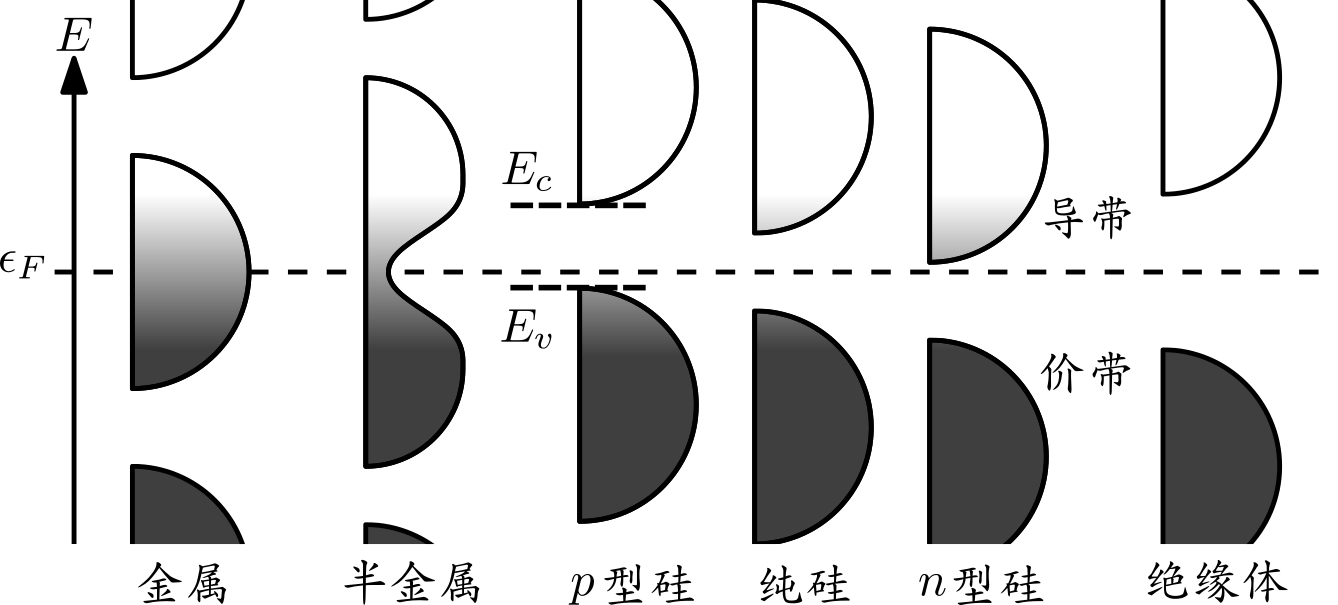
\includegraphics[width=.75\linewidth]{Band_filling.png}
	\caption[能带示意图]{金属、半导体、绝缘体的能带示意图\footnote{%
		示意图据开源资源修改得到:
		\url{https://en.wikipedia.org/wiki/File:Band_filling_diagram.svg}
	}}\vspace{1ex}
	\raggedright\small
	\textit{\hphantom{说明}
		$E_c,E_v$分别为导带下界、价带上界;图中令各类材料具有一致的费米能,以比较各类材料$E_c,E_v$以及$E_g = E_c - E_v$的相对大小。
	\vspace{1ex}}
	\label{fig:bandFilling}
	\end{figure}
	
	参见\cite{textbook}, 固体理论给出的电导率$\sigma$随温度$T$变化规律如下:
	\begin{enumerate}
	\item \textit{低温}:杂质部分电离,$p\sim p_s < N_A$, $n$很小,杂质散射主导,$\sigma \sim ep\mu_p$; 迁移率$\mu_p$随温度的变化并不显著,综合有
		$\pdv{\sigma}{T} > 0$; 
	\item 升温直到\textit{杂质饱和电离},但本征激发尚不强时,$p\sim p_s = N_A$, $n$依然很小,$\sigma \sim eN_A\mu_p$; 但此时晶格散射开始主导,电子--声子相互作用导致迁移率显著下降,因此
		$\pdv{\sigma}{T} < 0$; 
	这一阶段的变化规律与导体类似;
	\item \textit{较高温度}:本征激发显著,成对地产生电子、空穴,$n,p$均随温度指数增大,$p = p_s + n = N_A + n$; 迁移率依然为下降趋势,但仅仅是按幂律减小,故最终结果为$\sigma$增大,
		$\pdv{\sigma}{T} > 0$. 
	\end{enumerate}
	由于$\rho = \frac{1}{\sigma}$, 其随温度的变化规律与$\sigma$相反;温度增大,$\rho$先增后减再增。
	
	进一步,考虑本征激发占优的阶段(\textit{即上述讨论的\tup{c.}阶段}),室温$T_0 \sim \SI{300}{\kelvin}$对应的热激发能量量级为:
	\begin{equation}
		k T_0 \sim \SI{.03}{\eV}
	\end{equation}
	其中$k = k_\tup{B}$为玻尔兹曼常量,而半导体能隙$E_g$在 \SI{1}{\eV} 量级	(\textit{能级间隔的典型尺度,或参见\cite{morin1954electrical}}),有$E_g \gg kT_0$, 可采用玻尔兹曼分布描述粒子数按能量的分布:
	\begin{equation}
	\begin{aligned}
		a_n(\epsilon) &\sim \exp\pqty{
			\frac{\epsilon_F - \epsilon}{kT}},\quad
		&\epsilon \ge E_c\colon\,\textit{导带能量下界}\\[1ex]
		a_p(\epsilon) &\sim \exp\pqty{
			\frac{\epsilon - \epsilon_F}{kT}},\quad
		&\epsilon \le E_v\colon\,\textit{价带能量上界}
	\end{aligned}
	\end{equation}
	这里利用了费米子的泡利不相容原理:$a_p + a_n = 1$, 进一步积分可得:
	\begin{equation}
		np \propto T^3\,e^{-\frac{E_g}{kT}}
	\end{equation}
	也就是说,可根据本征激发阶段的$\sigma(T)$函数关系推断半导体的能隙:
	\begin{equation}
		E_g = \frac{\Delta\ln\pqty{npT^{-3}}}
			{\Delta\frac{1}{kT}}
		\label{eq:energyGap}
	\end{equation}
\subsection{霍尔效应}
	磁场与电流方向正交时,洛伦兹力导致正、负载流子分别沿
		${}\pm\hat{\vb{I}}\times\hat{\vb{B}}$
	方向运动,在导体的侧面(宽度记为$d$)处累积电荷;平衡时的电压即霍尔电压$V_H$, 有:
	\begin{equation}
		V_H = v_d B \ell
	\end{equation}
	导体的几何结构如图 \ref{fig:HallApp} 所示。
\clearpage
	
	\begin{figure}[!h]
	\vspace{.8ex}
	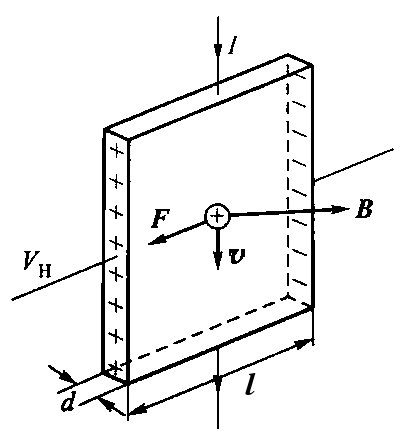
\includegraphics[width=.45\linewidth]{HallApp.jpg}
	\caption[霍尔元件示意图]{霍尔元件示意图,参见\cite{textbook}.}
	\vspace{1ex}
	\raggedright\small
	\textit{\hphantom{说明}
		这里绘制的是带正电载流子的情形,此时$\vb{v}_d$与$\hat{\vb{I}}$同向。对带负电载流子而言,$\vb{v}_d$与$\hat{\vb{I}}$反平行;固定电流方向不变,这将导致积累到图中宽为$d$的侧面的电荷类型发生变化,$V_H$正负发生改变。
	\vspace{1ex}}
	\label{fig:HallApp}
	\end{figure}
	
	可见,$I_p = pe\cdot Av_d,\,I_n = -ne\cdot Av_d$, 其中$A = w\ell$为电流截面积,这导致:
	\begin{equation}
		V_H = R_H\,\frac{IB}{d},\quad
		R_H =
		\left\lbrace
		\begin{aligned}
			\frac{1}{pq},\quad
				&\textit{载流子统一带正电荷$(+e)$}\\[1ex]
			-\frac{1}{nq},\quad
				&\textit{载流子统一带负电荷$(-e)$}
		\end{aligned}
		\right.
	\end{equation}
	对于同时具有正、负载流子的半导体而言,需要考虑叠加效应;由于空穴、电子的迁移率不同,这将导致两者的$v_d$不一致,不能简单地将$p,n$的贡献相加;参见 \cite{kasap2001hall}, 更为细致的分析表明,近似有:
	\begin{equation}
		R_H = \frac{3\pi}{8e} \frac{p-nb^2}{(p+nb)^2},\quad
		b = \frac{\mu_n}{\mu_p}
		\label{eq:hallRh}
	\end{equation}
	这里$1 < b \sim \order{1}$, 即电子的迁移率高于空穴,但两者近似处于同一量级。
	
	在此基础上,可简要分析$R_H$随$T$增大的变化规律:
	\begin{enumerate}
	\item 在强磁场、极低温下,上述讨论是不完备的,需要考虑更为丰富的量子效应;对特定的材料,可能出现\textit{量子霍尔效应},本文暂不对此进行讨论;
	\item 在较低温时,杂质电离饱和(\textit{对应前述电导变化的\tup{b}. 阶段}),此时$p\gg n$, $b\sim\order{1}$, 此时载流子几乎全为空穴且浓度不变,有$R_H \sim \tup{const.} > 0$. 
	\item 升温直至本征激发开始,此时$n$显著增大,导致$R_H$随温升而不断减小,直到$p\sim nb^2$时,$R_H = 0$. 进一步升温,$R_H$变为负值,即此后电子对$R_H$的贡献占优;
	\item 再升温,本征激发使载流子数目指数增大,$p = n + N_A \sim n$, 根据 \eqref{eq:hallRh}, 这表明$R_H$将指数减小,最终$R_H \to 0$. 
	\end{enumerate}
	
	上述$\tup{c.}\to\tup{d.}$阶段的过渡表明,在$R_H < 0$区域$R_H$将取到一极值;利用$p = n + N_A$及 \eqref{eq:hallRh}, 可得:
	\begin{equation}
		(R_H)_{\min}
		= R_H\Big|_{n = \frac{N_A}{b-1}}
		= -R_{H,s} \frac{(b-1)^2}{4b},\quad
		R_{H,s} = - \frac{3\pi}{8e} \frac{1}{N_A}
		\label{eq:bValueEstimated}
	\end{equation}
	注意这里的$R_{H,s}$恰是杂质电离饱和区的霍尔系数,可由此估算$b$值。
\section{实验装置}
%%	在此部分需要将实验条件交待清楚到别人能重复你的实验结果的程度. 此外,还需表明你已尽了最大努力来提高实验精度和结果的可靠性. 简单的不确定度估计可以在此节给出,复杂一些的可以放到分析讨论部分.\par
%%	实验条件不仅是指直接影响实验结果的实验参量,而且还包括影响实验质量和可靠性的因素,如室温、空气湿度、基真空、原材料纯度等.\par
%%	作为教学实验报告,此节写详细一点没有坏处.\par
%%	成段有叙述,必要才分节。
%%%%%%%%%%%%%%%%%%%%%%%%%%%%%%%
	本实验中的磁场由永磁环提供,大小$B \simeq \SI{.402}{\tesla}$; 为测定及计算方便,采用恒流$I = \SI{100.00(2)}{\uA}$. 所采用p型硅样品厚度$d = \SI{1.00(2)}{\mm}$. 
	
	样品加热以及供电、测温、测压电路集成封装于BWH-1型霍尔效应测试仪当中;样品温度采用温差电偶\footnote{%
		本实验采用铜--康铜热电偶,电势
		$\frac{\varepsilon}{\si{\mV}}
			= at + bt^2 + ct^3,\,
			t = \frac{T}{\si{\kelvin}} - 273$, \\
		参数$a = \num{3.827e-2},\,
			b = \num{5.59e-5},\,
			c = \num{-1.06e-7}$. 
	}测得。由于温度分布并不均匀,测定过程中势必存在温差电动势、热磁效应等诸多副效应;通过电流、磁场换向测定并加以平均,
	可以消除大部分副效应\footnote{%
		详尽的细致分析参见 \cite{textbook}, 此处不再重复。
	}。
	
	\begin{figure}[!h]
	\vspace{-2ex}
	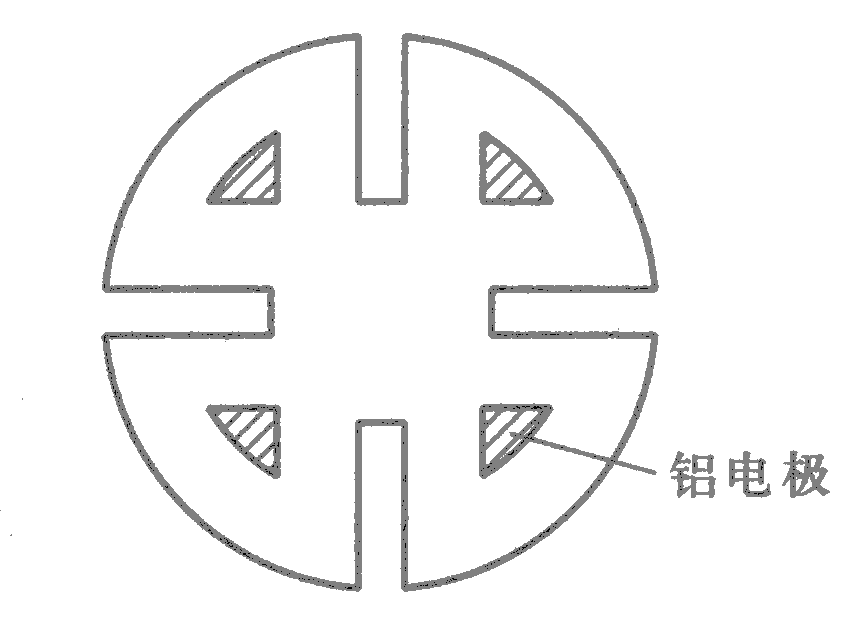
\includegraphics[width=.35\linewidth]{specSi.png}
	\caption[实验样品示意]{实验采用的p型硅样品示意图,
		参见\cite{textbook}.}
	\label{fig:specSi}
	\vspace{-1ex}
	\end{figure}
	本实验中的样品制成均匀的四叶薄片,可以认为通电后样品内部的电流密度$\vb{j}$为二维分布,电阻率$\rho$处处相等;此时电流分布可以在复平面$\mbb{C}$上分析处理:
	\[ \vb{j}\sim j = j_x + \mrm{i} j_y \]
	根据连续性方程和欧姆定律($\vb{j} = \sigma\vb{E}$),可知$j = j(z)$实际为复平面上的解析函数,$z = x + \mrm{i}y$; 只要该区域无空洞(\textit{单连通}),据黎曼映射定理,可将该区域上的电流分布保角变换到上半平面内求解。这一绝妙而优雅的方案首先由范德堡(van der Pauw)提出\supercite{van1958method}, 本实验即采用这一办法测定$\rho$和$R_H$. 参见 \cite{van1958method}, 
	\begin{equation}
		\rho = \frac{\pi d}{\ln 2}
			\frac{R_{12,34} + R_{23,41}}{2} f,\quad
		R_H = \frac{d}{B} \Delta R_{13,24}
	\end{equation}
	其中 (1,2,3,4) 为触点的编号,$\Delta$表示加磁场前后的变化;$f \le 1$是对称性因子,对本实验采用的样品,有$f\sim 1$. 在此基础上开始测定。
\section{结果与分析}
%	实验结果应尽量以图表的形式给出. 每一个图表都应该是完整的,即阅读图表时可以不必依赖正文.\par
%	依自己意愿,实验结果和对结果的分析讨论既可分为两节也可合在一节.\par
%
%	每个图一般包含:图名、轴名、轴、刻度、标尺、数据点、曲线、图例、标注和图注等部分. 应尽量让读者不看正文就能基本理解图的含意.\par
%	逐点测量得到的函数关系要同时用表格和图给出. 需要作比较的多条曲线要画在同一图上.\par
%	为避免读者在图表和正文间反复跳跃阅读,在正文中也要对图表作必要的说明.\par
%
%	对于预料之外的实验结果,必须首先小心证明其可靠性.读者只有在相信你的实验结果时才愿意花时间看你的分析.\par
%	必须用文字归纳整理出正式的实验结果或结论.可信的实验结果是课程报告最重要的内容.作为一个实验物理工作者,分析解释出错并不丢脸,实验结果不被采信则是致命的.\par
%	教学实验的结论往往是预先知道的. 所以,教师更关心的是你的说理过程. 一般说来,单由课内实验的结果不足以能得到明确的结论. 此时,你可以引用他人的研究结果来帮助帮助自己的论证,但必须注明出处. \par
%	确实不能得到明确结论时,可以给出几种可能结论并指出可以再做哪些实验来帮助作进一步的判断.\par
%	总之,分析讨论部分要做到: 论据要valid,论证要reasonable,结论要convincing.\par
%%%%%%%%%%%%%%%%%%%%%%%%%%%%%%
	实验中,观察到加热器到样品的热平衡弛豫时间很长;此外,固定加热器的设定温度,观察到样品的温度先增后减。由于加热器由反馈电路控制,不断调整工作状态(\textit{时开时关}),实际的热流为一振荡的波动;推测长时间看来,样品的温度也具有振荡的行为,需要很长时间才能最终达到平衡。
\clearpage
	
	为提高测定效率,同时保证测定时间内样品的温度近似恒定,本实验中的读数在近平衡态下进行;具体而言,采用如下读数策略:
	\begin{enumerate}[label=\arabic*.]
	\item 调整加热器设定温度后,观察样品温度的变化;当样品温度$T$达到峰值附近(\textit{几乎不变,或略有下降})时读数。此时样品的温度变化最为缓慢,近似为平衡态。
	\item 一组读数完成后,再次获取样品温度$T'$, 要求读数前后:
		\[ \frac{\Delta T}{T} = \frac{T' - T}{T}
			\lesssim 1\% \]
	便认为这组数据有效,否则进一步等待并重复前述步骤\tup{a}, 重新读取该组数据,直到满足这一条件为止。最终结果如图 \ref{fig:rhoRhSimple} 所示。	
	\end{enumerate}
	
	考察图线变化,与固体理论的分析比较,可见图线体现了前述分析中的\tup{b.}及后续阶段;具体而言,有:
	\begin{enumerate}[labelindent=\parindent,leftmargin=0pt,align=left]
	\item[$\tup{b.}\to \tup{c.}$] 室温($\sim\SI{25}{\celsius}$)至$\sim \SI{70}{\celsius}$范围内,$\rho$增大,表明杂质电离达到饱和,晶格散射占主导;$R_H$略减,表明此时本征激发实际已经开始,只是尚不显著;
	\item[c.] \SIrange{70}{120}{\celsius}, $\rho,R_H$锐减,可见本征激发开始显著影响电导和载流子成分,$\rho$降至 \SI{1000}{\ohm\cdot\cm} 附近,而$R_H$跨越零点降至负值;
	\item[d.] \SIrange{120}{150}{\celsius}, 本征激发占绝对主导地位,$\rho$继续减小但变化趋势缓慢,而$R_H$达到负的极值后转而趋近于零,与前述理论分析一致。
	\end{enumerate}
\subsection{杂质饱和区}
	前述分析表明此时的$\sigma \sim eN_A\mu_p$, 故$\rho(T) = \frac{1}{\sigma}$函数实际反应了$\mu(T)$关系。这里采用\cite{textbook}给出的参考值:
	\[ \mu_p|_{\SI{300}{\K}} = \SI{480}{\cm^2/(V\cdot\sec)} \]
	$\ln\rho = - \ln\pqty{eN_A} - \ln\mu_p$, 
	作对数图线,可更清晰地反映这一函数关系;参见图 \ref{fig:rhoRhLog}. 
	
	\begin{figure}[p]
	\centering
	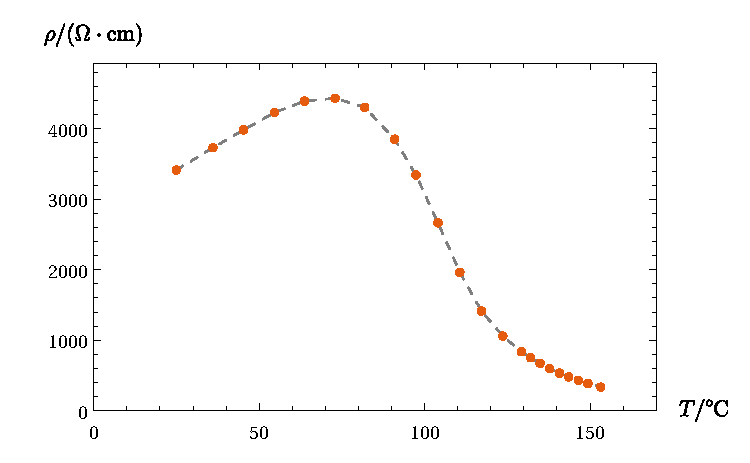
\includegraphics[width=.85\linewidth]{tempRhoPlot.pdf}\\
	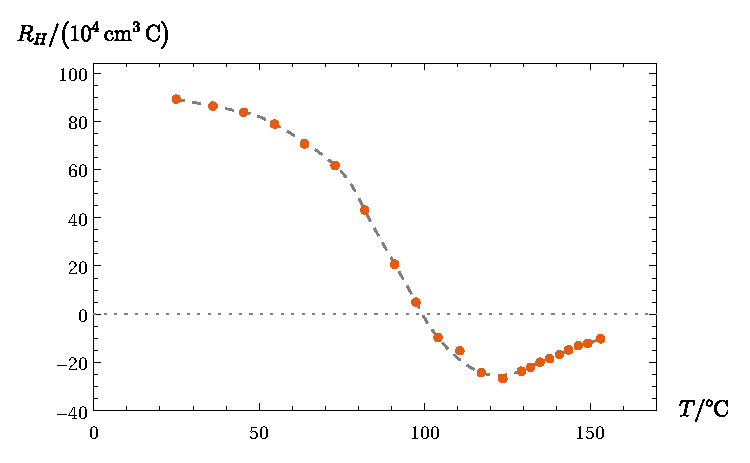
\includegraphics[width=.85\linewidth]{tempHallPlot.pdf}
	\caption[实测图]{实测电阻率$\rho$, 霍尔系数$R_H$示意图}
	\vspace{1ex}
	\raggedright\small
	\textit{\hphantom{说明}
		这里采用摄氏温标,以便于直观分析。$\rho$--$T$曲线的变化规律较为简单,其趋势线(图中虚线)由线性插值给出;$R_H$--$T$曲线的变化相对复杂,且在 \SI{100}{\celsius} 附近$R_H$由正转负,其趋势线(图中虚线)由三次样条插值给出。
	\vspace{1ex}}
	\label{fig:rhoRhSimple}
	\end{figure}
	
	\begin{figure}[p]
	\centering
	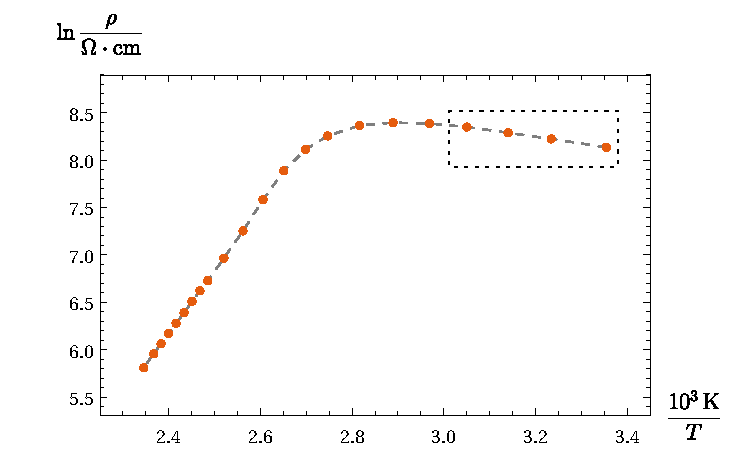
\includegraphics[width=.85\linewidth]{tempRhoLog.pdf}\\
	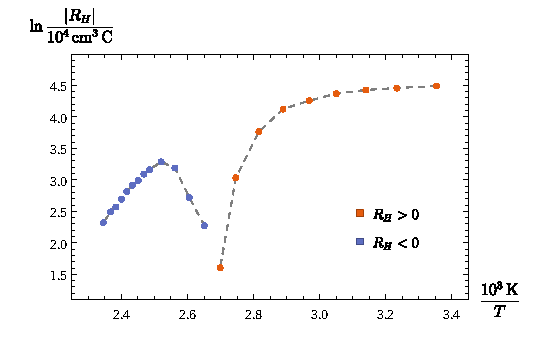
\includegraphics[width=.85\linewidth]{tempHallLog.pdf}
	\caption[实测对数图]{实测电阻率$\rho$, 霍尔系数$R_H$示意图,
		采用对数--$\frac{1}{T}$标度. }
	\vspace{1ex}
	\raggedright\small
	\textit{\hphantom{说明}
		这里采用绝对温标 \si{\K}, 以便于定量计算;曲线的趋势(图中虚线)均由线性插值给出。$R_H \gtrless 0$的情况分段作于同一图中;两段曲线不能简单地合为同一曲线,这是因为$R_H = 0$时$\ln|R_H| \to -\infty$奇异,即$\ln|R_H|$本身便不是连续曲线,分段考虑方为合理。此外,选取用于线性拟合的数据点以方框圈出。
	\vspace{1ex}}
	\label{fig:rhoRhLog}
	\end{figure}
	
	取图示四点进行线性拟合,可得杂质饱和区内,有:
	\begin{equation}
		\ln\frac{\rho}{\si{\ohm\cdot\cm}}
		= (\num{10.87(7)})
			+ (\num{2.26(6)})\,\ln\frac{T}{\SI{e3}{\K}}
	\end{equation}
	相关性系数$R^2 \simeq 0.9987$足够好,进一步设$\mu_p = A\,\pqty\big{T/\si{\K}}^{-x}$, 得:
	\begin{equation}
		x = \num{2.26(6)}
	\end{equation}
	
	这里引用 \cite{morin1954electrical} 给出的参考值:
	\begin{equation}
		\frac{\mu_p}{\si{\cm^2/(V\cdot\sec)}}
		= \num{2.5e8}\,\pqty\big{T/\si{\K}}^{-2.3}
		\label{eq:morinMobility}
	\end{equation}
	可见指数部分大致吻合;进一步引用 \cite{textbook} 提供的参考值
	$\mu_p|_{\SI{300}{\K}}$, 可得比例系数:
	\begin{equation}
		\num{1.9e8} \le
		\frac{A}{\si{\cm^2/(V\cdot\sec)}} \le 
		\num{2.7e8}
	\end{equation}
	$A$的可取范围很大,这是因为指数$x$上的微小误差被显著地放大了;考虑不确定度,\cite{morin1954electrical}的参考值落在实测所允许的范围之内,可以认为两者大致吻合。
	
	此外,本实验给出的测定值\CJKunderdot{势必}与精确值有所偏离;事实上,根据前面关于$R_H$变化规律的分析可见,室温下实际已经有少许的本征激发(\textit{从而$R_H$随温度减小}),因此$\sigma \sim eN_A\mu_p$并不严格成立。
	
	为获得更加精确的测定值,应当考察室温以下的$\rho(T), R_H(T)$关系,选取$R_H \simeq \mrm{const.}$的区域进行分析;这在本次实验中未能实现,可作为后续进一步实验的目标。由于本实验中未能得到更为精确的$\mu_p(T)$关系,后续计算将在 \cite{morin1954electrical} 给出的式 \eqref{eq:morinMobility} 基础上进行;例如,结合拟合式可外推得$\rho|_{\SI{300}{\K}} \simeq \SI{3475}{\ohm.\cm}$, 从而有:
	\begin{equation}
		N_A \simeq \SI{3.6e12}{\cm^{-3}}
	\end{equation}
\subsection{本征激发区}
	此时$\frac{1}{\rho} = \sigma
		= e\pqty{p\mu_p + n\mu_n}$, 
	同样引用 \cite{morin1954electrical}, 有
		$b \sim 16.0\times (T/\si{\K})^{-0.3}$; 
	考察最高测量温度时的测定值,
	\[ T_{\max} \simeq \SI{153.2}{\celsius},\quad
		\rho \simeq \SI{333.0}{\ohm\cdot\cm},\quad
		R_H \simeq \SI{-1.02e5}{\cm^3.\coulomb} \]
	结合前已求出的$N_A \simeq \SI{3.6e12}{\cm^{-3}}$, 可得:
	\begin{equation}
		p|_{\SI{153.2}{\celsius}} \simeq
		\SI{2.6e13}{\cm^{-3}}
	\end{equation}
	
	由上可见,$p = n + N_A \gg N_A$, 或$n \gg N_A$, 高出一个数量级,表明此时确已充分进入本征激发范围。
	
	\newparagraph
	据$b \sim 16.0\times (T/\si{\K})^{-0.3}$, 可得在室温至$T_{\max}$的范围内,有:
	\begin{equation}
		b \in \pqty{2.60,2.98}
	\end{equation}
	可见$b$随温度缓变,可以独立于 \cite{morin1954electrical}, 据前述式 \eqref{eq:bValueEstimated} 估计 \SI{120}{\celsius} 附近的$b$值。这里选用实测数据点:
	\[ T_{\max} \simeq \SI{123.6}{\celsius},\quad
		\rho \simeq \SI{1058.5}{\ohm\cdot\cm},\quad
		R_H \simeq \SI{-2.67e5}{\cm^3.\coulomb} \]
	作为$R_H$峰值的一个估计,利用 \eqref{eq:bValueEstimated}, 可得
		$b \simeq 2.02$. 
	显然这个估计值是比较差劲的,但至少在数量级上没有出错;究其原因,大概是由于$N_A$误差较大,其根源依然是$\rho(T)$关系的拟合不够精准,应增加低于室温情况下的测量数据,以提高精度。
\subsection{能隙计算}
	\vspace{-.5\baselineskip}
	根据前述理论分析,作$\ln p$及$\ln\frac{np}{T^3}$随温度变化的图线,结果如下。
	\begin{figure}[!h]
	\vspace{-1ex}
	\centering
	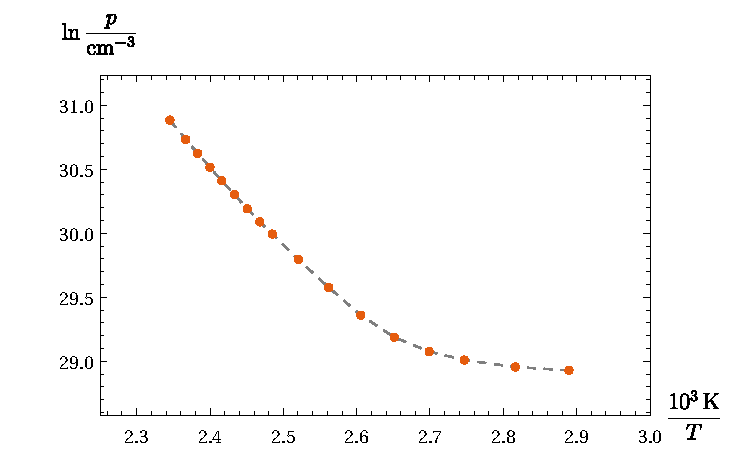
\includegraphics[width=.8\linewidth]{logPplot.pdf}\\
	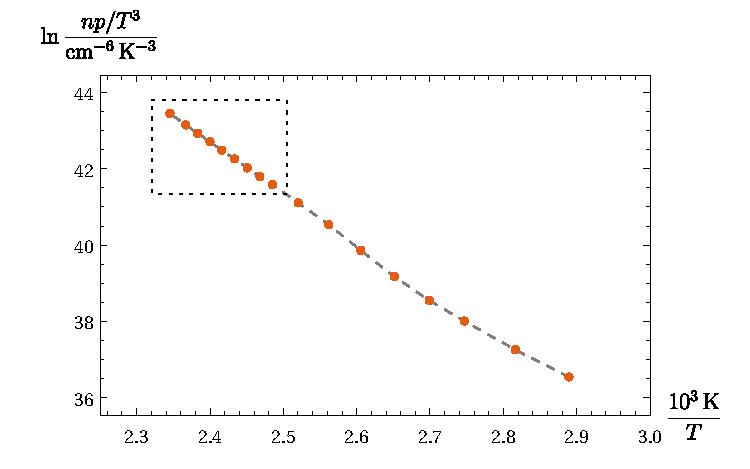
\includegraphics[width=.8\linewidth]{logNPplot.pdf}
	\caption[载流子浓度对数图]{%
		载流子浓度随温度变化的对数图像}
	\vspace{1ex}
	\raggedright\small
	\textit{\hphantom{说明}
		这里采用绝对温标 \si{\K}, 以便于定量计算;曲线的趋势(图中虚线)均由线性插值给出。图中仅包含本征激发阶段的温度范围,即大于 \SI{70}{\celsius} 的温度区域。此外,选取用于线性拟合的数据点以方框圈出。
	\vspace{-3ex}}
	\label{fig:logNP}
	\end{figure}
	
	选取方框区域线性拟合,得斜率:
	\begin{equation}
		\frac{\Delta\ln\pqty{npT^{-3}}}
			{\Delta\frac{1}{kT}} \simeq \num{-1.3e4}
	\end{equation}
	相关性系数$R^2 = 0.9998$足够好,利用 \eqref{eq:energyGap}, 这给出:
	\begin{equation}
		E_g \simeq \SI{1.12}{\eV}
	\end{equation}
\section{结论}
%%%	首先要给出实验结果,然后再给出由实验结果分析得到的结果和结论.此部分给出的内容要比摘要中的全面,用词要更准确.\par
%%%%%%%%%%%%%%%%%%%%%%%%%%%%%%%
	实验测得了室温以上至$\sim\SI{150}{\celsius}$范围内p型硅电阻率与霍尔系数随温度的变化趋势,由此初步验证了固体理论对描述半导体的有效性。实验结果表明,取用的p型硅样品在室温下已处于杂质电离饱和区,随后电学特性随温度变化的规律与固体理论的预测一致。
	
	在此基础上,实验估算了p型硅的杂质浓度和本征激发充分时的载流子浓度,两者分别在 \SI{e12}{\cm^{-3}} 和 \SI{e13}{\cm^{-3}} 量级;同时验证了$\mu_p(T)$的函数关系,基本与 \cite{morin1954electrical} 一致。进一步,实验给出了电子、空穴迁移率比例$b$的估计值,确认有$1 < b \sim \order{1}$; 最终测得禁带宽度约为 \SI{1.12}{\eV}. 
\section{致谢}
%	此部分感谢同组人...和对实验和报告有帮助的人.
%%%%%%%%%%%%%%%%%%%%%%%%%%%%%%
	感谢与我合作的李征儒学长,尤其感谢他在读数时的出色工作;感谢耐心的吴孝松老师给我们带来的启发和巨大帮助。
\clearpage

\setlength{\bibsep}{2pt}
\linespread{1.2}\selectfont
\bibliographystyle{../BibStyle/gbt-7714-2015-numerical}
\bibliography{../BibStyle/Textbook,bib/Ref}

\clearpage
\end{document}
